% !TeX root = ../../main.tex
\chapter{Tehnologii folosite}
\label{cap:tehnologii}

\section{Angular}

\subsection{Prezentare generală -- Single Page Application}
Angular este un framework frontend dezvoltat de Google pentru aplicații web de tip SPA (Single Page Application), unde interfața se actualizează dinamic fără reîncărcarea completă a paginii. Într-un SPA, browserul încarcă inițial aplicația (HTML, CSS, JavaScript), iar apoi navigarea internă se face prin rutare la nivel de client și apeluri către API pentru date, nu prin încărcarea repetată a unor pagini complete de pe server \cite{google_angular_2024,takada_spa_2024}.

Comparativ cu tehnologiile web mai vechi, de tip MPA (Multi-Page Application) sau server-side rendering clasic în care fiecare acțiune importantă trimite o cerere nouă și primește un document HTML complet, modelul SPA are mai multe avantaje practice: latență percepută mai mică la navigare, interacțiuni mai fluide (fără "flash" de reîncărcare), posibilitatea de a păstra starea în interfață (filtre, tab-uri, formulare parțial completate), și separarea clară între frontend și backend. În plus, aceeași API poate deservi mai multe tipuri de clienți (web, mobile), ceea ce simplifică evoluția sistemului pe termen lung \cite{sciencedirect_client_server_2026,aws_restful_2024}.

Din perspectiva dezvoltării, ecosistemul modern completează foarte bine modelul SPA. De exemplu, Vite este un tool de dezvoltare și build axat pe pornire rapidă și actualizări instant în timpul codării, folosind module native și un mecanism performant de HMR (Hot Module Replacement). Conceptual, HMR (denumit frecvent și "hot swap" în limbaj informal) permite înlocuirea modulelor modificate fără refresh complet al paginii, păstrând pe cât posibil starea aplicației și accelerând ciclul editare--testare. Chiar dacă în acest proiect frontend-ul este construit cu Angular CLI, principiul este același: feedback rapid în dezvoltare și productivitate crescută în aplicații SPA complexe \cite{google_angular_cli_2026,vite_docs_2026,vite_hmr_2026}.

Fluxul de lucru specific Vite + HMR este ilustrat în Figura~\ref{fig:vite-hmr-flow}.

\begin{figure}[H]
	\centering
	\includegraphics[width=0.9\textwidth]{images/vite-hmr-flow.png}
	\caption{Flux Vite + Hot Module Replacement (HMR)}
	\label{fig:vite-hmr-flow}
\end{figure}

În practică, fluxul din figură funcționează astfel: dezvoltatorul modifică un fișier (componentă, stil sau modul), serverul Vite detectează schimbarea și recompilă doar partea afectată, apoi transmite actualizarea către browser prin canalul activ de dezvoltare. Browserul înlocuiește modulul modificat fără reîncărcare completă a paginii, ceea ce reduce timpul de feedback și, în multe cazuri, păstrează starea curentă a interfeței (de exemplu date deja introduse în formular). Acest mecanism este motivul principal pentru care experiența de dezvoltare în aplicațiile SPA moderne este mai rapidă și mai fluidă.

\subsection{Angular Command Line Interface -- comenzi \texttt{ng}}
Angular Command Line Interface este instrumentul oficial care automatizează întreg ciclul de viață al aplicației Angular: creare proiect, generare fișiere, rulare locală, testare și compilare pentru producție. Rolul său principal este standardizarea proiectului și reducerea timpului de configurare manuală, astfel încât dezvoltarea să rămână concentrată pe funcționalități, nu pe configurare tehnică \cite{google_angular_cli_2026}.

Un aspect important este că modul de execuție al comenzilor poate fi configurat din fișierul \texttt{angular.json}, unde sunt definite țintele de compilare și rulare, opțiunile pentru medii diferite, directoarele de ieșire, resursele statice și alte setări de construcție ale aplicației.

În continuare sunt prezentate comenzile cele mai importante folosite în practică.

\subsubsection{\texttt{ng new} -- inițializarea proiectului}
Comanda \texttt{ng new} creează un proiect Angular complet, cu fișierele de configurare, structura directoarelor și dependențele necesare. Este punctul de pornire pentru orice aplicație nouă.

\begin{lstlisting}[language=bash]
ng new student-management-frontend --routing --style=scss
\end{lstlisting}

În acest exemplu, \texttt{--routing} activează suportul pentru rutare, iar \texttt{--style=scss} setează formatul principal pentru stiluri.

\subsubsection{\texttt{ng serve} -- rularea în dezvoltare}
\texttt{ng serve} pornește serverul local de dezvoltare și compilează aplicația în mod incremental. La fiecare salvare, modificările sunt detectate automat și reflectate rapid în browser.

\begin{lstlisting}[language=bash]
ng serve
ng serve --open
\end{lstlisting}

Această comandă este folosită continuu în timpul implementării, deoarece oferă răspuns imediat asupra erorilor și modificărilor din interfață.

\subsubsection{\texttt{ng build} -- compilarea pentru producție}
\texttt{ng build} generează versiunea optimizată a aplicației pentru publicare pe server. În modul de producție sunt aplicate minificarea și optimizarea pachetelor de cod.

\begin{lstlisting}[language=bash]
ng build --configuration production
\end{lstlisting}

Rezultatul final este plasat în directorul \texttt{dist/}, care reprezintă versiunea publicabilă pe server \cite{google_angular_cli_2026}.

\subsubsection{\texttt{ng generate} -- generarea de componente și servicii}
Comanda \texttt{ng generate} creează automat fișiere conform convențiilor Angular: componente, servicii, directive sau pipe-uri. Astfel se reduce codul repetitiv și se menține consistența structurii.

\begin{lstlisting}[language=bash]
ng generate component features/students/student-list
ng generate service shared/services/student
\end{lstlisting}

\subsubsection{\texttt{ng add} -- integrarea bibliotecilor}
\texttt{ng add} nu doar instalează un pachet, ci aplică și configurări automate necesare integrării în proiect (acolo unde biblioteca oferă mecanisme de generare automată).

\begin{lstlisting}[language=bash]
ng add @angular/material
\end{lstlisting}

Această abordare reduce riscul de configurare incompletă comparativ cu o instalare manuală simplă prin comanda \texttt{npm install}.

\subsubsection{\texttt{ng test} -- testarea automată}
Comanda \texttt{ng test} rulează testele unitare ale aplicației și oferă feedback rapid privind corectitudinea componentelor și serviciilor.

\begin{lstlisting}[language=bash]
ng test
\end{lstlisting}

Într-un flux profesional, testarea este executată periodic pe durata dezvoltării, pentru a detecta devreme regresiile introduse în cod \cite{google_angular_cli_2026}.

\subsection{Directive -- folosite pentru afișare condiționată}
Directivele sunt mecanismul prin care Angular controlează felul în care este construită și actualizată interfața. Practic, ele spun ce se afișează, cum se afișează și cum reacționează elementele la datele din aplicație. În practică, directivele se împart în trei categorii: componente, directive de atribut și directive structurale \cite{google_angular_2024,angular_directives_2026}.

\subsubsection{1. Componente (directive cu șablon propriu)}
Acesta este tipul folosit cel mai des. Fiecare componentă Angular este, tehnic, o directivă care are propriul șablon, propria logică și propriile stiluri. Prin componente, interfața este împărțită în părți mici și reutilizabile, ceea ce face codul mai ușor de organizat și de întreținut.

Exemplu:

\begin{lstlisting}[language=HTML]
<app-user-profile></app-user-profile>
\end{lstlisting}

\subsubsection{2. Directive de atribut}
Directivele de atribut se aplică pe un element existent și îi schimbă stilul sau comportamentul, fără să îi elimine ori să îi adauge noduri în Modelul de Obiect al Documentului. Sunt utile atunci când aceeași regulă vizuală sau funcțională trebuie reutilizată în mai multe zone ale aplicației.

Câteva directive folosite frecvent în Angular:
\begin{itemize}
		\item \texttt{NgClass} -- adaugă sau elimină clase de stil în funcție de starea componentei;
		\item \texttt{NgStyle} -- adaugă sau elimină stiluri în linie;
		\item \texttt{NgModel} -- permite legarea bidirecțională a datelor în elementele de formular.
\end{itemize}

Exemplu scurt cu \texttt{NgClass}:

\begin{lstlisting}[language=HTML]
<span [ngClass]="{'activ': esteActiv, 'inactiv': !esteActiv}">
  Status cont
</span>
\end{lstlisting}

Exemplu de directivă personalizată de atribut (denumire mai sugestivă: \texttt{appHoverAccent}):

\begin{lstlisting}[language=HTML]
<p appHoverAccent>Treci cu mouse-ul peste acest text</p>
\end{lstlisting}
\newpage
Exemplu scurt de implementare:

\begin{lstlisting}[language=TypeScript]
import { Directive, ElementRef, HostListener } from '@angular/core';

@Directive({
	selector: '[appHoverAccent]'
})
export class HoverAccentDirective {
	constructor(private elementRef: ElementRef) {}

	@HostListener('mouseenter')
	onMouseEnter(): void {
		this.elementRef.nativeElement.style.backgroundColor = '#e8f4ff';
		this.elementRef.nativeElement.style.transition = 'background-color 0.2s ease';
	}

	@HostListener('mouseleave')
	onMouseLeave(): void {
		this.elementRef.nativeElement.style.backgroundColor = '';
	}
}
\end{lstlisting}

\subsubsection{3. Directive structurale}
Directivele structurale influențează direct structura șablonului: pot adăuga, elimina sau repeta elemente. De aceea, ele sunt folosite când interfața depinde de condiții sau de colecții de date. În sintaxa clasică, apar frecvent cu prefixul \texttt{*}.

Cele mai întâlnite exemple sunt:
\begin{itemize}
		\item \texttt{*ngIf} -- include un șablon doar dacă o condiție este adevărată;
		\item \texttt{*ngFor} -- repetă un element pentru fiecare obiect dintr-o colecție;
		\item \texttt{*ngSwitch} -- selectează una dintre mai multe variante de afișare.
\end{itemize}
Exemplu scurt cu \texttt{*ngIf} și \texttt{*ngFor}:

\begin{lstlisting}[language=HTML]
<p *ngIf="esteAutentificat">Bun venit in aplicatie!</p>

<ul>
  <li *ngFor="let student of studenti">{{ student.nume }}</li>
</ul>
\end{lstlisting}

Exemplu scurt cu \texttt{*ngSwitch}:

\begin{lstlisting}[language=HTML]
<div [ngSwitch]="rolUtilizator">
  <p *ngSwitchCase="'admin'">Panou de administrare</p>
  <p *ngSwitchCase="'student'">Pagina studentului</p>
  <p *ngSwitchDefault>Rol necunoscut</p>
</div>
\end{lstlisting}

\subsection{Arhitectura pe componente}
Arhitectura Angular este bazată pe componente reutilizabile, fiecare componentă având logică TypeScript, șablon HTML și stiluri dedicate. În locul unui fișier foarte mare care gestionează toată interfața, aplicația este împărțită în unități mici, fiecare responsabilă pentru o zonă clară din ecran. Această separare face codul mai ușor de înțeles, testat și extins \cite{google_angular_2024}.

Într-o aplicație de dimensiune medie sau mare, componentele sunt organizate de obicei pe niveluri:
\begin{itemize}
	\item componente de pagină (de exemplu: lista studenților, pagina de cursuri, pagina de prezență);
	\item componente de funcționalitate (de exemplu: tabel de rezultate, formular de editare, filtru de căutare);
	\item componente partajate (de exemplu: buton reutilizabil, mesaj de eroare, dialog de confirmare).
\end{itemize}

Un avantaj important al acestei arhitecturi este comunicarea controlată între componente. Datele curg de la părinte la copil prin \texttt{@Input}, iar evenimentele urcă de la copil la părinte prin \texttt{@Output}. Astfel, fluxul devine predictibil, iar dependențele dintre părți rămân clare.

Elementul central este decoratorul \texttt{@Component}, unde sunt definite metadatele componentei. Cele mai importante proprietăți sunt:
\begin{itemize}
	\item \texttt{selector} -- numele etichetei HTML prin care componenta este folosită în alte șabloane;
	\item \texttt{templateUrl} sau \texttt{template} -- sursa șablonului (fișier separat sau șablon scris direct în cod);
	\item \texttt{styleUrl} sau \texttt{styles} -- sursa stilurilor (fișier separat sau stiluri inline).
\end{itemize}

Varianta recomandată pentru componente mai mari folosește fișiere separate:

\begin{lstlisting}[language=TypeScript]
@Component({
	selector: 'app-student-list',
	templateUrl: './student-list.component.html',
	styleUrl: './student-list.component.scss'
})
export class StudentListComponent {
	@Input() students: Student[] = [];
}
\end{lstlisting}

Această abordare oferă separare clară între logică, structură și stiluri, fiind mai ușor de întreținut atunci când componenta crește.

Folosirea selectorului împreună cu \texttt{@Input} în componenta părinte:

\begin{lstlisting}[language=HTML]
<app-student-list [students]="studentiActivi"></app-student-list>
\end{lstlisting}

În acest exemplu, \texttt{app-student-list} este selectorul componentei copil, iar proprietatea \texttt{studentiActivi} din părinte este transmisă către \texttt{@Input() students}.

Pentru componente mici, se poate folosi șablon și stil direct în decorator:

\begin{lstlisting}[language=TypeScript]
@Component({
	selector: 'app-status-badge',
	template: '<span class="badge">{{ text }}</span>',
	styles: ['.badge { padding: 4px 8px; border-radius: 6px; }']
})
export class StatusBadgeComponent {
	@Input() text = 'Activ';
}
\end{lstlisting}

Varianta inline este rapidă și utilă pentru componente foarte simple, dar pentru componente reale, cu structură mai mare, varianta cu \texttt{templateUrl} și \texttt{styleUrl} rămâne mai clară și mai scalabilă.

În practică, componentele păstrează logica de prezentare, iar operațiile de date (apeluri către server, mapări de date, reguli comune) sunt mutate în servicii injectabile. Această delimitare între prezentare și logică de business reduce duplicarea și crește mentenabilitatea pe termen lung.

\subsection{Rutare}
Rutarea în Angular definește harta de navigare a aplicației: ce componentă se încarcă pentru fiecare adresă și ce reguli de acces se aplică pe fiecare zonă. În aplicații mai mari, rutarea nu este doar navigare între pagini, ci și un mecanism de organizare a modulelor, de control al accesului și de separare pe niveluri funcționale \cite{google_angular_2024}.

O practică uzuală este definirea unei rute părinte pentru zona protejată (de exemplu \texttt{/dashboard}) și a unor rute copil pentru funcționalități (studenți, cursuri, prezență). Astfel, structura adreselor rămâne coerentă, iar componentele comune (layout, meniu lateral, antet) se declară o singură dată în componenta părinte.

\begin{lstlisting}[language=TypeScript]
export const routes: Routes = [
	{ path: 'login', component: LoginComponent },
	{
		path: 'dashboard',
		component: DashboardLayoutComponent,
		children: [
			{ path: 'students', component: StudentsPageComponent },
			{ path: 'courses', component: CoursesPageComponent },
			{ path: 'attendance', component: AttendancePageComponent },
			{ path: '', redirectTo: 'students', pathMatch: 'full' }
		]
	},
	{ path: '', redirectTo: 'login', pathMatch: 'full' }
];
\end{lstlisting}

Proprietatea \texttt{children} permite gruparea rutelor care aparțin aceleiași secțiuni. Beneficiul major este reutilizarea layout-ului părinte și păstrarea unei ierarhii clare a adreselor, de tip \texttt{/dashboard/students} sau \texttt{/dashboard/attendance}.

Pentru eficientizarea încărcării inițiale, Angular permite și încărcarea la cerere a componentelor prin \texttt{loadComponent}. În această abordare, componenta nu este inclusă în pachetul inițial al aplicației, ci este descărcată doar când utilizatorul accesează ruta respectivă. Astfel se evită încărcarea inutilă a componentelor care nu sunt folosite imediat după autentificare, iar timpul de pornire perceput al aplicației scade.

\begin{lstlisting}[language=TypeScript]
{
	path: 'attendance',
	loadComponent: () =>
		import('./features/attendance/attendance-page.component')
			.then(m => m.AttendancePageComponent)
}
\end{lstlisting}

În același timp, gărzile de rută verifică dacă utilizatorul are voie să acceseze o rută înainte de încărcarea componentei. În mod tipic, un guard verifică existența sesiunii (token valid) și redirecționează utilizatorul spre pagina de autentificare dacă accesul nu este permis.

\begin{lstlisting}[language=TypeScript]
export const authGuard: CanActivateFn = () => {
	const authService = inject(AuthService);
	const router = inject(Router);

	if (authService.isAuthenticated()) {
		return true;
	}

	return router.createUrlTree(['/login']);
};
\end{lstlisting}

Un exemplu de aplicare a guard-ului pe rută este prezentat mai jos:

\begin{lstlisting}[language=TypeScript]
{
	path: 'dashboard',
	component: DashboardLayoutComponent,
	canActivate: [authGuard],
	children: [
		{ path: 'students', component: StudentsPageComponent }
	]
}
\end{lstlisting}

Legătura dintre rutare și componentele vizuale se face prin \texttt{router-outlet}, care reprezintă zona în care Angular afișează componenta asociată rutei active. În practică, navigarea între rute este realizată în șablon prin \texttt{routerLink}, fără reîncărcarea completă a paginii.

\begin{lstlisting}[language=HTML]
<nav>
	<a routerLink="/dashboard/students">Studenti</a>
	<a routerLink="/dashboard/courses">Cursuri</a>
</nav>

<router-outlet></router-outlet>
\end{lstlisting}

Pentru scenarii în care o pagină trebuie să afișeze date în funcție de un identificator, ruta poate primi parametri. De exemplu, pentru detaliile unui student, configurația poate include un parametru de tip \texttt{:id}, iar componenta îl citește din \texttt{ActivatedRoute}.

\begin{lstlisting}[language=TypeScript]
{ path: 'students/:id', component: StudentDetailsComponent }

const id = this.route.snapshot.paramMap.get('id');
\end{lstlisting}

În practică, navigarea dintre componente se face frecvent direct din cod TypeScript, nu doar din șablon. Pentru acest lucru se folosește \texttt{Router}, iar \texttt{ActivatedRoute} oferă contextul rutei curente. Combinația dintre cele două este utilă în scenarii precum: redirecționare după salvare, trecere la următorul element din listă sau schimbarea unei subrute în cadrul aceleiași pagini.

\begin{lstlisting}[language=TypeScript]
constructor(
	private router: Router,
	private route: ActivatedRoute
) {}

goToStudent(id: number): void {
	this.router.navigate(['../', id], { relativeTo: this.route });
}
\end{lstlisting}

Exemplul de mai sus folosește navigare relativă, ceea ce înseamnă că noua adresă este construită pornind de la ruta curentă. Această abordare reduce dependența de căi absolute scrise manual și face mai simplă refactorizarea structurii de rute.

Un aspect important este că \texttt{snapshot} citește parametrii o singură dată. Dacă utilizatorul rămâne pe aceeași componentă, iar parametrul se schimbă (de exemplu de la \texttt{/students/10} la \texttt{/students/11}), este recomandat să se folosească fluxul reactiv al parametrilor:

\begin{lstlisting}[language=TypeScript]
this.route.paramMap.subscribe(params => {
	const id = params.get('id');
	// reincarca datele in functie de id
});
\end{lstlisting}

În același mod pot fi transmise și informații suplimentare prin \texttt{queryParams}, de exemplu pentru tab-uri, filtre sau paginare:

\begin{lstlisting}[language=TypeScript]
this.router.navigate(['students', id], {
	queryParams: { tab: 'attendance', page: 1 }
});
\end{lstlisting}

În plus, o rută wildcard este folosită pentru adrese necunoscute, evitând situațiile în care utilizatorul rămâne pe o pagină goală sau într-o stare necontrolată. De regulă, wildcard-ul redirecționează către o pagină de autentificare sau către o pagină de tip "nu a fost găsit".

\begin{lstlisting}[language=TypeScript]
{ path: '**', redirectTo: 'login' }
\end{lstlisting}

Prin combinarea ierarhiei de rute, a rutelor copil și a gărzilor de acces, aplicația obține o navigare clară, sigură și ușor de extins pe termen lung.

\subsection{Formulare}
Angular oferă două abordări principale pentru formulare: \textit{template-driven forms} și \textit{reactive forms}. Prima abordare este mai simplă și potrivită pentru formulare mici, unde regulile sunt puține și logica este directă. A doua abordare este recomandată pentru aplicații mai mari, deoarece oferă control explicit asupra structurii formularului, a validărilor și a fluxului de submit \cite{google_angular_2024}.
În aplicația realizată au fost folosite ambele abordări: \textit{template-driven forms} pentru formulare scurte și simple, respectiv \textit{reactive forms} pentru formulare cu reguli multiple de validare și fluxuri mai complexe.

În cazul formularelor \textit{template-driven}, structura se definește în principal în șablonul HTML, folosind directiva \texttt{ngModel} și referințe locale de tip \texttt{ngForm}. Această abordare este utilă pentru ecrane simple (de exemplu formular de contact sau autentificare minimală), unde logica de validare este redusă și se dorește implementare rapidă.

\begin{lstlisting}[language=HTML]
<form #loginForm="ngForm" (ngSubmit)="onLogin(loginForm)">
	<input
		type="email"
		name="email"
		[(ngModel)]="model.email"
		required
		email
		#email="ngModel"
	/>

	<div *ngIf="email.invalid && email.touched">
		<small *ngIf="email.errors?.['required']">Email-ul este obligatoriu.</small>
		<small *ngIf="email.errors?.['email']">Format email invalid.</small>
	</div>

	<button type="submit" [disabled]="loginForm.invalid">Autentificare</button>
</form>
\end{lstlisting}

În această variantă, starea formularului (valid, invalid, touched) este gestionată automat de Angular pe baza atributelor declarate în template. Pentru formulare mici, codul rămâne ușor de citit, însă pe măsură ce numărul de câmpuri și reguli crește, mentenanța devine mai dificilă decât în abordarea reactivă.

În practica aplicațiilor de management, formularele reactive sunt preferate deoarece permit definirea câmpurilor și a validatorilor în TypeScript, ceea ce face codul mai ușor de testat și întreținut. Un exemplu tipic este definirea unui formular cu câmpuri obligatorii, validare de format pentru email și lungime minimă pentru parolă:

\begin{lstlisting}[language=TypeScript]
form = this.fb.group({
	email: ['', [Validators.required, Validators.email]],
	password: ['', [Validators.required, Validators.minLength(8)]],
	fullName: ['', [Validators.required]]
});
\end{lstlisting}

Validarea este eficientă atunci când utilizatorul primește feedback clar și la momentul potrivit. În interfață, mesajele de eroare sunt afișate de regulă după ce câmpul a fost atins sau modificat, pentru a evita o experiență agresivă la prima încărcare a paginii.

\begin{lstlisting}[language=HTML]
<input type="email" formControlName="email" />

<div *ngIf="form.get('email')?.invalid && form.get('email')?.touched">
	<small *ngIf="form.get('email')?.errors?.['required']">
		Email-ul este obligatoriu.
	</small>
	<small *ngIf="form.get('email')?.errors?.['email']">
		Formatul email-ului este invalid.
	</small>
</div>
\end{lstlisting}

Partea de submit trebuie să valideze formularul înainte de trimiterea datelor către server. Dacă formularul nu este valid, toate câmpurile sunt marcate ca atinse pentru a afișa erorile relevante. Dacă formularul este valid, se transmite doar obiectul de valori și se tratează răspunsul de succes sau eroare.

\begin{lstlisting}[language=TypeScript]
onSubmit(): void {
	if (this.form.invalid) {
		this.form.markAllAsTouched();
		return;
	}

	this.studentService.createStudent(this.form.value).subscribe({
		next: () => {
			// notificare succes si reset formular
			this.form.reset();
		},
		error: () => {
			// notificare eroare
		}
	});
}
\end{lstlisting}

Prin această structură, validarea din frontend reduce datele incorecte trimise către server, iar utilizatorul primește feedback imediat, coerent și ușor de înțeles.

\subsection{Servicii injectabile}
Serviciile injectabile sunt folosite pentru logica partajată (de exemplu, autentificare, acces la API, utilitare), separând responsabilitățile de prezentare din componente. Mecanismul de \textit{Dependency Injection} permite furnizarea serviciilor într-un mod centralizat și testabil \cite{google_angular_2024}.

În practică, o componentă nu ar trebui să conțină direct apeluri HTTP sau reguli comune reutilizate în mai multe ecrane. Aceste responsabilități sunt mutate în servicii, iar componenta rămâne concentrată pe interacțiunea cu utilizatorul și afișarea datelor. Această separare reduce duplicarea, simplifică testarea unitară și face codul mai ușor de extins.

Într-o aplicație de management studențesc, serviciile apar în mod natural pe zone funcționale: \texttt{StudentsService}, \texttt{CoursesService}, \texttt{AttendanceService}, \texttt{AuthService}. Fiecare serviciu expune metode clare pentru operații de tip listare, creare, actualizare sau ștergere, iar componentele folosesc aceste metode fără a cunoaște detaliile endpoint-urilor.

Un avantaj major este centralizarea tratării erorilor și a transformărilor de date. De exemplu, același format de eroare venit de la API poate fi mapat într-un mesaj prietenos pentru interfață într-un singur loc, nu duplicat în fiecare componentă.

Un tipar uzual este injectarea serviciului în constructorul componentei și apelarea metodelor dedicate pentru încărcare sau salvare date:

\begin{lstlisting}[language=TypeScript]
@Injectable({ providedIn: 'root' })
export class StudentsService {
	constructor(private http: HttpClient) {}

	getAll(): Observable<Student[]> {
		return this.http.get<Student[]>('/api/students/list.php');
	}
}

@Component({
	selector: 'app-students-page',
	templateUrl: './students-page.component.html'
})
export class StudentsPageComponent {
	students: Student[] = [];

	constructor(private studentsService: StudentsService) {}
}
\end{lstlisting}

În plus, serviciile injectabile permit reutilizarea aceleiași logici în mai multe componente. De exemplu, lista de studenți poate fi folosită atât în pagina de administrare, cât și în pagina de prezență, fără duplicare de cod. Astfel, orice modificare de endpoint sau regulă de mapare se face o singură dată în serviciu și se propagă în tot frontend-ul.

Un exemplu practic pentru operația de creare, cu tratare minimă a erorilor, este:

\begin{lstlisting}[language=TypeScript]
createStudent(payload: CreateStudentDto): Observable<Student> {
	return this.http.post<Student>('/api/students/create.php', payload).pipe(
		catchError((error: HttpErrorResponse) => {
			const message = error.status === 409
				? 'Studentul exista deja.'
				: 'A aparut o eroare la salvare.';
			return throwError(() => new Error(message));
		})
	);
}
\end{lstlisting}

\subsection{RxJS -- pentru gestionare evenimente}
RxJS (Reactive Extensions for JavaScript) este o bibliotecă externă folosită de Angular pentru lucrul cu date asincrone. În Angular 19, \texttt{HttpClient} returnează \texttt{Observable}, iar componentele se abonează la aceste fluxuri prin \texttt{subscribe} \cite{rxjs_team_2024,google_angular_2024}.

\begin{figure}[H]
	\centering
	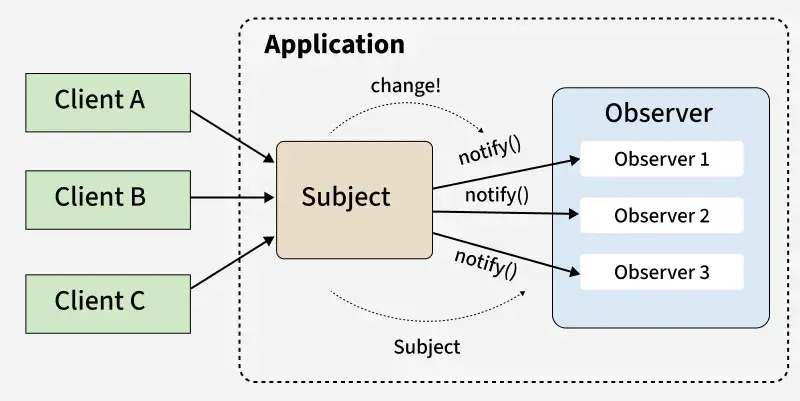
\includegraphics[width=0.72\textwidth]{images/observer-design-Pattern.png}
	\caption{Modelul RxJS în Angular: Observable și Subscriber}
	\label{fig:rxjs-observable-subscriber}
\end{figure}

Pe scurt, un \texttt{Observable} este sursa care emite date în timp, iar \texttt{Subscriber}-ul este componenta care primește acele date. Metoda \texttt{subscribe} pornește consumul fluxului.

În acest context, \texttt{ngOnInit} și \texttt{ngOnDestroy} aparțin ciclului de viață al componentei și sunt utile pentru gestionarea subscripțiilor:
\begin{itemize}
	\item \texttt{ngOnInit} -- momentul potrivit pentru inițierea subscripției;
	\item \texttt{ngOnDestroy} -- momentul potrivit pentru oprirea subscripției.
\end{itemize}

Exemplu simplu, ușor de urmărit:

\begin{lstlisting}[language=TypeScript]
import { Component, OnInit, OnDestroy } from '@angular/core';
import { Subscription } from 'rxjs';

@Component({
	selector: 'app-attendance-page',
	templateUrl: './attendance-page.component.html'
})
export class AttendancePageComponent implements OnInit, OnDestroy {
	private attendanceSub?: Subscription;
	rows: Attendance[] = [];

	constructor(private attendanceService: AttendanceService) {}

	ngOnInit(): void {
		this.attendanceSub = this.attendanceService
			.getBySession(12)
			.subscribe(data => {
				this.rows = data;
			});
	}

	ngOnDestroy(): void {
		this.attendanceSub?.unsubscribe();
	}
}
\end{lstlisting}

Prin această abordare, componenta pornește încărcarea datelor la inițializare și eliberează corect resursele la distrugere, evitând subscripții rămase active.

\subsection{Interceptor}
Interceptorul este un mecanism Angular care interceptează fiecare cerere HTTP înainte să plece spre server și fiecare răspuns înainte să ajungă în componentă. Rolul lui principal este să centralizeze logică transversală (cross-cutting), astfel încât componentele și serviciile să rămână curate și concentrate pe funcționalitatea de business \cite{google_angular_2024,mdn_http_2026}.

În aplicația de față, interceptorul este util în special pentru:
\begin{itemize}
	\item atașarea automată a token-ului JWT în header-ul \texttt{Authorization};
	\item tratarea unitară a erorilor de autentificare (de exemplu cod \texttt{401});
	\item logare/monitorizare pentru cereri și răspunsuri.
\end{itemize}

\begin{figure}[H]
	\centering
	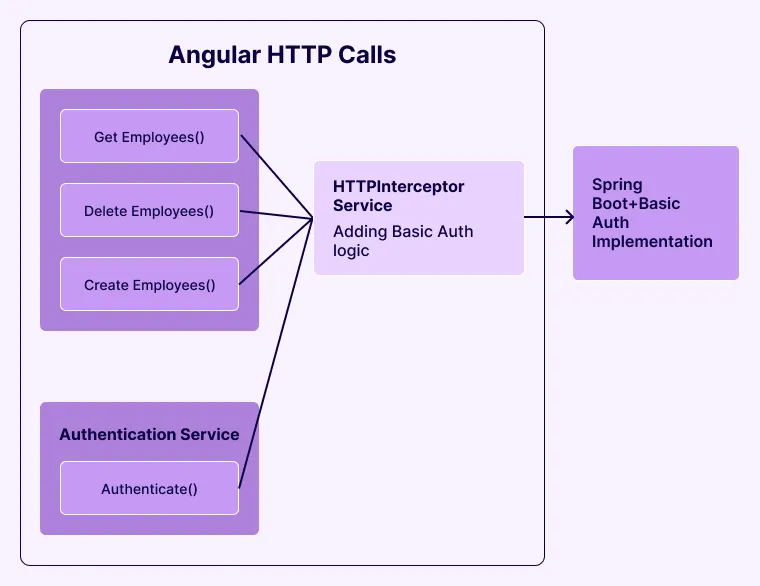
\includegraphics[width=0.78\textwidth]{images/interceptor.png}
	\caption{Poziționarea interceptorului între aplicația Angular și API}
	\label{fig:angular-interceptor-flow}
\end{figure}

În Angular 19, interceptorul poate fi introdus în configurația aplicației prin \texttt{provideHttpClient} și \texttt{withInterceptors}. Astfel, el devine activ global pentru toate apelurile realizate prin \texttt{HttpClient}.

\begin{lstlisting}[language=TypeScript]
import { HttpInterceptorFn } from '@angular/common/http';

export const authInterceptor: HttpInterceptorFn = (req, next) => {
	const token = localStorage.getItem('token');

	const authReq = token
		? req.clone({
			setHeaders: { Authorization: `Bearer ${token}` }
		})
		: req;

	return next(authReq);
};
\end{lstlisting}

Pe scurt, interceptorul reduce duplicarea (nu mai adăugăm manual token-ul în fiecare serviciu), crește consistența comunicării cu backend-ul și simplifică mentenanța pe termen lung.

\subsection{UI -- Angular Material + Bootstrap + Icons}
Interfața aplicației combină Angular Material, Bootstrap și o bibliotecă de iconuri pentru a obține o experiență vizuală coerentă, responsivă și ușor de folosit. Fiecare tehnologie are un rol clar: Angular Material oferă componente UI standardizate, Bootstrap oferă sistemul de layout și utilitare CSS rapide, iar iconurile cresc lizibilitatea acțiunilor importante \cite{angular_material_2026,bootstrap_docs_2026,bootstrap_icons_2026}.

Angular Material -- de ce este folosit. Angular Material este folosit pentru componente reutilizabile precum tabele, dialoguri, câmpuri de formular, butoane și notificări. Avantajul principal este consistența vizuală între ecrane și reducerea timpului de implementare.

Integrarea în proiect se poate realiza cu:

\begin{lstlisting}[language=bash]
ng add @angular/material
\end{lstlisting}

După instalare, componentele necesare se importă în aplicație, iar în template sunt utilizate direct:

\begin{lstlisting}[language=HTML]
<mat-form-field appearance="outline">
	<mat-label>Email</mat-label>
	<input matInput type="email" />
</mat-form-field>

<button mat-raised-button color="primary">Salvare</button>
\end{lstlisting}

Bootstrap -- de ce este folosit. Bootstrap este folosit în principal pentru grid, spațiere, aliniere și responsive behavior. În acest mod, paginile rămân ușor de adaptat pe desktop, tabletă și mobil, fără CSS extins pentru fiecare ecran.

Instalare și integrare uzuală:

\begin{lstlisting}[language=bash]
npm install bootstrap
\end{lstlisting}

Fișierul CSS Bootstrap este apoi inclus în stilurile globale ale aplicației (de exemplu în \texttt{styles.css} sau în configurația \texttt{angular.json}). Utilizarea în template este directă, prin clase:

\begin{lstlisting}[language=HTML]
<div class="container mt-3">
	<div class="row g-3">
		<div class="col-12 col-md-6">Panou studenti</div>
		<div class="col-12 col-md-6">Panou cursuri</div>
	</div>
</div>
\end{lstlisting}

Icons -- de ce sunt folosite. Iconurile sunt folosite pentru acțiuni repetitive (editare, ștergere, căutare, export), deoarece reduc timpul de recunoaștere vizuală și fac interfața mai clară.

Un mod frecvent este folosirea Bootstrap Icons:

\begin{lstlisting}[language=bash]
npm install bootstrap-icons
\end{lstlisting}

După includerea fișierului CSS al iconurilor în stilurile globale, acestea se folosesc direct în template:

\begin{lstlisting}[language=HTML]
<button class="btn btn-outline-primary btn-sm">
	<i class="bi bi-pencil-square"></i>
	Editare
</button>
\end{lstlisting}

Prin această combinație, interfața devine mai rapid de implementat, mai uniformă vizual și mai ușor de întreținut pe termen lung.

\section{Modelul Client-Server}

\subsection{Protocolul HTTP}
Modelul client-server separă responsabilitățile între client (interfața utilizator) și server (logica de business și accesul la date). Comunicare între cele două părți se realizează, în mod standard, prin protocolul HTTP, folosind metode precum \texttt{GET}, \texttt{POST}, \texttt{PUT} și \texttt{DELETE} \cite{sciencedirect_client_server_2026,mdn_http_2026}.

\subsection{JSON}
JSON este formatul de schimb de date folosit în API-urile web datorită simplității și interoperabilității sale. În arhitectura client-server, serverul trimite frecvent răspunsuri JSON, iar clientul serializează/deserialiează datele pentru afișare și prelucrare \cite{json_org_2026}.

\section{PHP}

\subsection{Conectarea la baza de date}
În backend, PHP gestionează conectarea la MySQL prin extensii precum PDO, oferind suport pentru interogări parametrizate și tratamentul erorilor. Folosirea interogărilor parametrizate reduce riscul de SQL injection și crește securitatea accesului la date \cite{php_group_2024,oracle_mysql_2024}.

\subsection{Autentificare}
Autentificarea în API verifică identitatea utilizatorului pe baza credențialelor și emite un mecanism de acces pentru cererile ulterioare. În aplicațiile moderne, acest mecanism este de regulă stateless și bazat pe token-uri \cite{php_group_2024,jwt_io_2026}.

\subsubsection{JWT}
JWT (JSON Web Token) este un format standard pentru transmiterea securizată a informațiilor despre utilizator între client și server. După autentificare, token-ul este trimis de client în header-ul \texttt{Authorization} pentru accesarea rutelor protejate \cite{jwt_io_2026}.

\subsubsection{Validare}
Validarea datelor se aplică atât la autentificare (format email, parolă, existență utilizator), cât și la celelalte endpoint-uri API. Aceasta previne introducerea de date invalide în sistem și contribuie la robustețea aplicației \cite{php_group_2024}.

\subsection{Structura fișiere pentru API}
O structură organizată pe directoare (de exemplu: autentificare, studenți, cursuri, prezență) simplifică mentenanța și extinderea backend-ului. Separarea endpoint-urilor de configurații și modele permite o mai bună claritate a responsabilităților în cod \cite{php_group_2024}.

\subsection{Stocare fișiere}
Pentru fișiere încărcate de utilizatori, o practică uzuală este păstrarea în baza de date doar a căii (\textit{path}), iar fișierul fizic în directoare dedicate, de tip \texttt{/uploads/X}. Această abordare reduce dimensiunea tabelelor, simplifică backup-ul și permite control mai bun al accesului la fișiere \cite{php_group_2024}.

\section{MySQL}

\subsection{Diagrama ER}
Modelarea bazei de date relaționale pornește de la diagrama Entitate-Relație (ER), care descrie entitățile, atributele și relațiile dintre ele. În contextul aplicației de management studențesc, diagrama ER clarifică legăturile dintre studenți, grupe, discipline, prezențe și programări de examene \cite{wikipedia_er_2026,oracle_mysql_2024}.

\section{Git}

Git este sistemul de versionare distribuit utilizat pentru urmărirea modificărilor din cod, colaborare și revenirea la versiuni stabile. Fluxurile bazate pe branch-uri și commit-uri facilitează dezvoltarea incrementală și controlul calității în proiecte software realizate în echipă \cite{git_doc_2026}.
